\documentclass[17pt]{beamer}
%\documentclass[handout]{beamer} %Makes Handouts
\usetheme{Singapore} %Gray with fade at top
\useoutertheme[subsection=false]{miniframes} %Supppress subsection in header
\useinnertheme{rectangles} %Itemize/Enumerate boxes
\usecolortheme{seagull} %Color theme
\usecolortheme{rose} %Inner color theme

\definecolor{light-gray}{gray}{0.75}
\definecolor{dark-gray}{gray}{0.55}
\setbeamercolor{item}{fg=light-gray}
\setbeamercolor{enumerate item}{fg=dark-gray}

\setbeamertemplate{navigation symbols}{}
\setbeamertemplate{mini frames}{}
%\setbeamercovered{dynamics}
\setbeamerfont*{title}{size=\Large,series=\bfseries}
\setbeamerfont{footnote}{size=\tiny}

%\setbeameroption{notes on second screen} %Dual-Screen Notes
%\setbeameroption{show only notes} %Notes Output

\setbeamertemplate{frametitle}{\vspace{.5em}\bfseries\insertframetitle}
\newcommand{\heading}[1]{\noindent \textbf{#1}\\ \vspace{1em}}
\newcommand{\questions}{\frame{{\large Questions?}}}

\usepackage{bbding,color,multirow,times,ccaption,tabularx,graphicx,verbatim,booktabs}
\usepackage{colortbl} %Table overlays
\usepackage[english]{babel}
\usepackage[latin1]{inputenc}
\usepackage[T1]{fontenc}
\usepackage{lmodern}
\usepackage{alltt}

\usepackage{tikz}
\usetikzlibrary{shapes,arrows,decorations.pathreplacing,calc}


\author[]{Thomas J. Leeper}
\institute{
  Government Department\\London School of Economics and Political Science
}


\title{Session I\\Survey Experiments in Context}

\date[]{}

\begin{document}

\frame{\titlepage}


\frame{\tableofcontents}


\frame{

\frametitle{Activity!}

\only<2-4,6>{
\begin{enumerate}
\item<2-4,6> Ask you to guess a number
\item<3-4,6> Number off 1 and 2 across the room
\item<4,6> Group 2, close your eyes
\item<6> Group 1, close your eyes
\end{enumerate}
}

\Large
\only<5>{\textit{Group 1}\\ Think about whether the population of Chicago is more or less than 500,000 people. What do you think the population of Chicago is?}
\only<7>{\textit{Group 2}\\ Think about whether the population of Chicago is more or less than 10,000,000 people. What do you think the population of Chicago is?}

}
\frame{}

\frame{

\frametitle{Enter your data}

\begin{itemize}\itemsep1em
\item Go here: \url{http://bit.ly/297vEdd}
\item Enter your guess and your group number
\end{itemize}

%\url{http://goo.gl/forms/xDW4FLm9pau0O8zz2}

}


\frame{

\frametitle{Results}

\begin{itemize}\itemsep1em
\item True population: 2.79 million
\item<2-> What did you guess? \href{https://docs.google.com/spreadsheets/d/1SKWljS1EeNkAV5V0NZUwrKOu3LQFILVMB37xfTxyrPM/edit?usp=sharing}{(See Responses)}
\item<3-> What's going on here?
	\begin{itemize}
	\item An experiment!
	\item Demonstrates ``anchoring'' heuristic
	\end{itemize}
\item<4-> Experiments are easy to analyze, but only if designed and implemented well
\end{itemize}

}



\section{Introductions}
\frame{\tableofcontents[currentsection]}

\frame{
\frametitle{Who am I?}

\small

\begin{itemize}\itemsep0.25em

\item Thomas Leeper

\item Assistant Professor in Political Behaviour at London School of Economics

\begin{itemize}
\item 2013--15: Aarhus University (Denmark)
\item 2008--12: PhD from Northwestern University (Chicago, USA)
\item Birth--2008: Minnesota, USA
\end{itemize}

\item Interested in public opinion and political psychology

\item Email: \href{mailto:t.leeper@lse.ac.uk}{t.leeper@lse.ac.uk}

\end{itemize}

}


\frame{

\frametitle{Who are you?}

\begin{itemize}\itemsep1em

\item Introduce yourself to a neighbour

\item Where are you from?

\item What do you hope to learn from the course?

\end{itemize}

}



\frame{

\frametitle{Quick Survey}

\begin{enumerate}\itemsep0.5em
\item<2-> How many of you have worked with survey data before?
\item<3-> Of those, how many of you have \textit{performed} a survey before?
\item<4-> How many of you have worked with experimental data before?
\item<5-> Of those, how many of you have \textit{performed} an experiment before?
\end{enumerate}

}



\section{Course Outline}
\frame{\tableofcontents[currentsection]}


\frame{

\frametitle{Course Materials}

\begin{center}
All material for the course is available at:\\

\vspace{1em}

\url{http://www.thomasleeper.com/surveyexpcourse/}
\end{center}

}

\frame{

\frametitle{Learning Outcomes}

\small

By the end of the week, you should be able to\dots

\begin{enumerate}
\item<2-> Explain how to analyze experiments quantitatively.
\item<3-> Explain how to design experiments that speak to relevant research questions and theories.
\item<4-> Evaluate the uses and limitations of several common survey experimental paradigms.
\item<5-> Identify practical issues that arise in the implementation of experiments and evaluate how to anticipate and respond to them.
\end{enumerate}

}


\frame{

\frametitle{Schedule of Four Sessions}

\begin{enumerate}\itemsep0.5em
\item Survey Experiments in Context
\item Examples and Paradigms
\item External Validity
\item Practical Issues
\end{enumerate}

}


\questions



\section[History]{History of Experiments}
\frame{\tableofcontents[currentsection]}

\frame{

\frametitle{Experiments}

Oxford English Dictionary defines ``experiment'' as:

\begin{enumerate}
\item A scientific procedure undertaken to make a discovery, test a hypothesis, or demonstrate a known fact
\item A course of action tentatively adopted without being sure of the outcome
\end{enumerate}
}

\frame{

\frametitle{Experiments}

\begin{itemize}\itemsep0.75em
\item ``Experiments'' have a very long history

\item Major advances in design and analysis of experiments based on agricultural and later biostatistical research in the 19th century
	\begin{itemize}
	\item R.A. Fisher
	\item Jerzy Neyman
	\item Karl Pearson
	\item Oscar Kempthorne
	\end{itemize}

\end{itemize}

}

\frame{

\frametitle{In Social Sciences}

\small

\begin{itemize}
\item ``Experiments'' emerged in psychology 19th century
	\begin{itemize}\footnotesize
	\item Not randomized -- more like ``What if?'' studies
	\item Heavily laboratory-based or clinical
	\end{itemize}
\item<2-> First randomized, controlled trial (RCT) by Peirce and Jastrow in 1884
\item<3-> RCTs came later to medicine (circa 1950)
\item<4-> And have been a major part of the ``credibility revolution'' in economics
	\begin{itemize}
	\item See, especially, LaLonde (1986)
	\end{itemize}
\end{itemize}

}


\frame{

\frametitle{In Social Science I}

\begin{itemize}\itemsep0.5em
\item APSA Pres. A. Lawrence Lowell (1922):\\
{\small
\textit{``We are limited by the impossibility of experiment. Politics is an observational, not an experimental science\dots''}
}
\item<2-> First experiment by Gosnell (1924)
\item<3-> Gerber and Green (2000) first major \textit{field} experiment
\end{itemize}

}

\frame{

\frametitle{{\large In Social Science II}}

\small

\begin{itemize}
\item Rise of surveys in the behavioral revolution
\item Survey research was not experimental because interviewing was still mostly paper-based
	\begin{itemize}
	\item ``Split Ballots'' (Schuman \& Presser; Bishop)
	\end{itemize}
\item<2-> 1983: Merrill Shanks and the Berkeley Survey Research Center develop CATI
\item<3-> Mid-1980s: Paul Sniderman \& Tom Piazza performed the first survey experiment\only<3->{\footnote{Sniderman, Paul M., and Thomas Piazza. 1993. \textit{The Scar of Race}. Cambridge, MA: Harvard University Press.}}
	\begin{itemize}\footnotesize
	\item Then: the ``first multi-investigator''
	\item Later: Skip Lupia and Diana Mutz created TESS
	\end{itemize}

\end{itemize}

}

\frame{

\frametitle{TESS}

\small

\begin{itemize}
\item Time-Sharing Experiments for the Social Sciences
\item Multi-disciplinary initiative that provides infrastructure for survey experiments on nationally representative samples of the United States population
\item Funded by the U.S. National Science Foundation
\item Anyone anywhere in the world can apply
\end{itemize}

}

\frame{

\frametitle{TESS-like Projects}

There are some TESS-like initiatives outside the United States:

\begin{itemize}\itemsep1em
\item Netherlands: \href{https://www.lissdata.nl/lissdata/}{LISS}
\item Norway: \href{http://www.uib.no/en/citizen}{Bergen's Citizen Panel}
\item Sweden: \href{http://lore.gu.se/surveys/citizen}{Gothenburg's Citizen Panel}
\end{itemize}

}


\questions



\section[Logic]{Logic and Analysis}
\frame{\tableofcontents[currentsection,subsubsectionstyle=hide]}


\frame{
	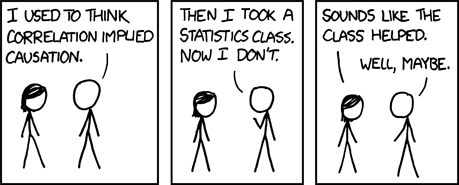
\includegraphics[width=\textwidth]{images/xkcdcorrelation.png}
}


\frame{

\frametitle{Addressing Confounding}

In observational research\dots

\begin{enumerate}\itemsep0.5em
\item<2-> Correlate a ``putative'' cause ($X$) and an outcome ($Y$)
\item<3-> Identify all possible confounds (\textbf{Z})
\item<4-> ``Condition'' on all possible confounds
	\begin{itemize}
	\item Calculate correlation between $X$ and $Y$ at each combination of levels of \textbf{Z}
	\end{itemize}
\item<5-> Basically: $Y = \beta_0 + \beta_1 X + \beta Z + \epsilon $
\end{enumerate}

}


\begin{frame}
\begin{center}
\begin{tikzpicture}[>=latex',circ/.style={draw, shape=circle, node distance=5cm, line width=1.5pt}]
    \draw (0,0) node[left] (X) {\textcolor<2->{red}{Smoking}};
    \draw[->] (X) -- (5,0) node[right] (Y) {Cancer};
    \draw[->] (-3,3) node[above] (Z) {Sex} -- (X);
    \draw[->] (Z) -- (Y);
    \draw[->] (5,2) node[above] (A) {Environment} -- (Y);
    \draw[->] (4,-3) node[below, text width=3cm, align=center] (E) {Genetic\\Predisposition} -- (Y);
    \draw[->] (-2, -2) node[below, text width=2.5cm, align=center] (W) {Parental\\Smoking} -- (X);
    \draw[->] (W) -- (Y);
    \draw<2->[->, dashed, very thick] (E) -- (X);
\end{tikzpicture}
\end{center}
\end{frame}




\frame{

\frametitle{Experiments are different}

\begin{enumerate}\itemsep0.75em
\item<2-> Draw causal inferences through \textit{design} not \textit{analysis}
\item<3-> Randomization breaks selection bias
\item<4-> We don't need to ``control'' for anything
\item<5-> We see ``causal effects'' in the comparison of experimental groups
\end{enumerate}

}


% Mill's method of difference
\frame{
\frametitle{{\normalsize Mill's Method of Difference}}

\small

If an instance in which the phenomenon under investigation occurs, and an instance in which it does not occur, \textbf<2->{have every circumstance save one in common}, that one occurring only in the former; \textbf<2->{the circumstance in which alone the two instances differ, is the} effect, or \textbf<2->{cause}, or an necessary part of the cause, \textbf<2->{of the phenomenon}.
}



\frame{

\frametitle{Definitions}

\only<2>{\textbf{Unit}: A physical object at a particular point in time}

\only<3>{\textbf{Treatment}: An intervention, whose effect(s) we wish to assess relative to some other (non-)intervention}

\only<4>{
\textbf{Potential outcomes}: The outcome for each unit that we would observe if that unit received each treatment
\begin{itemize}
\item Multiple potential outcomes for each unit, but we only observe one of them
\end{itemize}
}

\only<5>{\textbf{Causal effect}: The comparisons between the unit-level potential outcomes under each intervention}

}




% Individual-level effects versus ATEs


\frame{
	\frametitle{The Experimental Ideal}
	\small
	A randomized experiment, or randomized control trial is:
 		\begin{quote}\small
 			The observation of units after, and possibly before, a randomly assigned intervention in a controlled setting, which tests one or more precise causal expectations
 		\end{quote}
 	This is Holland's ``statistical solution'' to the fundamental problem of causal inference
}


\frame{
\frametitle{Two solutions!\footnote{From Holland}}

\begin{enumerate}\itemsep1em
\item Scientific Solution
	\begin{itemize}
	\item All units are identical
	\item Each can provide a perfect counterfactual
	\item Common in, e.g., agriculture, biology
	\end{itemize}
\item<2-> Statistical Solution
	\begin{itemize}
	\item Units are not identical
	\item Random exposure to a potential cause
	\item Effects measured on average across units
	\item Known as the ``Experimental ideal''
	\end{itemize}
\end{enumerate}

}



\frame{
\frametitle{The Experimental Ideal}
\begin{itemize}\itemsep0.5em
\item It solves both the temporal ordering and confounding problems of observational causal inference
	\begin{itemize}
   		\item Treatment ($X$) is applied by the researcher before outcome ($Y$)
   		\item Randomization means there are no confounding ($Z$) variables
	\end{itemize}
\item<2-> Thus experiments are a ``gold standard'' of causal inference
\item<3-> Basically: $Y = \beta_0 + \beta_1 X + \epsilon $
\end{itemize}
}


\frame{

\frametitle{Neyman--Rubin Potential Outcomes Framework}

If we are interested in some outcome $Y$, then for every unit $i$, there are numerous ``potential outcomes'' $Y*$ only one of which is visible in a given reality. Comparisons of (partially unobservable) potential outcomes indicate causality.

}

\frame{

\frametitle{Neyman--Rubin Potential Outcomes Framework}

Concisely, we typically discuss two potential outcomes:

\begin{itemize}\small
\item $Y_{0i}$, the \textit{potential} outcome \textit{realized} if $X_i = 0$ (b/c $D_i = 0$, assigned to control)
\item $Y_{1i}$, the \textit{potential} outcome \textit{realized} if $X_i = 1$ (b/c $D_i = 1$, assigned to treatment)
\end{itemize}

}


\frame{

\frametitle{Historical Aside}

\small

\begin{itemize}
\item The history of the potential outcomes framework is contested
\item Most people attribute it to Donald Rubin
\item Paul Holland was the first to link to the philosophical discussions of causality
\item Donald Rubin attributes this to Jerzy Neyman (1923)
\item James Heckman denies all of this and attributes it Andrew Roy (1951)
\end{itemize}
}







% design-based experimental inference
\frame{
	\frametitle{Experimental Inference I}
	\small
	\begin{itemize}\itemsep0.5em
    	\item<1-> Each unit has multiple \textit{potential} outcomes, but we only observe one of them, randomly
    	\item<2-> In this sense, we are sampling potential outcomes from each unit's population of potential outcomes
		\only<2->{
			\begin{center}
			\begin{tabular}{ccccc}
			unit & low & high & \onslide<3->{control} & \onslide<4->{etc.} \\ \midrule
			1 & ? & ? & \onslide<3->{?} & \onslide<4->{\dots} \\
			2 & ? & ? & \onslide<3->{?} & \onslide<4->{\dots} \\
			3 & ? & ? & \onslide<3->{?} & \onslide<4->{\dots} \\
			4 & ? & ? & \onslide<3->{?} & \onslide<4->{\dots} \\ \bottomrule
			\end{tabular}
			\end{center}
		}
	\end{itemize}
}

\frame{
	\frametitle{Experimental Inference II}
	\small
	\begin{itemize}\itemsep0.5em
    	\item<1-> We cannot see individual-level causal effects
    	\item<2-> We can see \textit{average causal effects}
    		\begin{itemize}
        		\item<2-> Ex.: Average difference in cancer between those who do and do not smoke
    		\end{itemize}
    	\item<3-> We want to know: $TE_i = Y_{1i} - Y_{0i}$
	\end{itemize}
}

\frame{
	\frametitle{Experimental Inference III}
	\small
	\begin{itemize}\itemsep0.5em
		\item<1-> We want to know: $TE_i = Y_{1i} - Y_{0i}$ for every $i$ in the population
		\item<2-> We can average: $E[TE_i] = E[Y_{1i} - Y_{0i}] = E[Y_{1i}] - E[Y_{0i}]$
		\item<3-> But we still only see one potential outcome for each unit:\\ \vspace{1em}
    		$ATE_{naive} = E[Y_{1i} | X = 1] - E[Y_{0i} | X = 0]$
    	\item<4-> Is this what we want to know?
	\end{itemize}
}


\frame{
	\frametitle{Experimental Inference IV}
	\small
	\begin{itemize}\itemsep0.5em
	\item What we want and what we have:
		\begin{align}
		ATE & = E[Y_{1i}] - E[Y_{0i}] \\[1em]
		ATE_{naive} & = E[Y_{1i} | X = 1] - E[Y_{0i} | X = 0]
		\end{align}		
	\item<2-> Are the following statements true?\\
  		\begin{itemize}\itemsep0.5em
      		\item<2-> $E[Y_{1i}] = E[Y_{1i} | X = 1]$
      		\item<2-> $E[Y_{0i}] = E[Y_{0i} | X = 0]$
  		\end{itemize}
  	\item<3-> Not in general!
  	\end{itemize}
}

\frame{
	\frametitle{Experimental Inference V}
	\small
	\begin{itemize}\itemsep0.5em
    	\item Only true when both of the following hold:
    	\begin{align}
    	E[Y_{1i}] = E[Y_{1i} | X = 1] = E[Y_{1i} | X = 0]\\
    	E[Y_{0i}] = E[Y_{0i} | X = 1] = E[Y_{0i} | X = 0]
    	\end{align}
    	\item In that case, potential outcomes are \textit{independent} of treatment assignment
		\item If true (e.g., due to randomization of $X$), then:
    	\begin{align*}
    	ATE_{naive} & = E[Y_{1i} | X = 1] - E[Y_{0i} | X = 0] \tag{5}\\
    	& = E[Y_{1i}] - E[Y_{0i}]\\
    	& = ATE
    	\end{align*}
	\end{itemize}
}

\frame{
	\frametitle{Experimental Inference VI}

	\normalsize
	\begin{itemize}\itemsep0.5em
    	\item This holds in experiments because of a \textit{physical process of randomization}\footnote{Random means ``known probability of treatment'' not ``haphazard''.}
   		\item<2-> Units differ only in side of coin that was up
	   		\begin{itemize}\footnotesize
	   		\item $X_i = 1$ only because $D_i = 1$
	   		\end{itemize}
	   	\item<3-> Implications:
		   	\begin{itemize}
		   	\item Covariate balance
		   	\item Potential outcomes balanced and independent of treatment assignment
		   	\item No confounding (selection bias)
		   	\end{itemize}
	\end{itemize}
}




\begin{frame}
\small 
\begin{center}
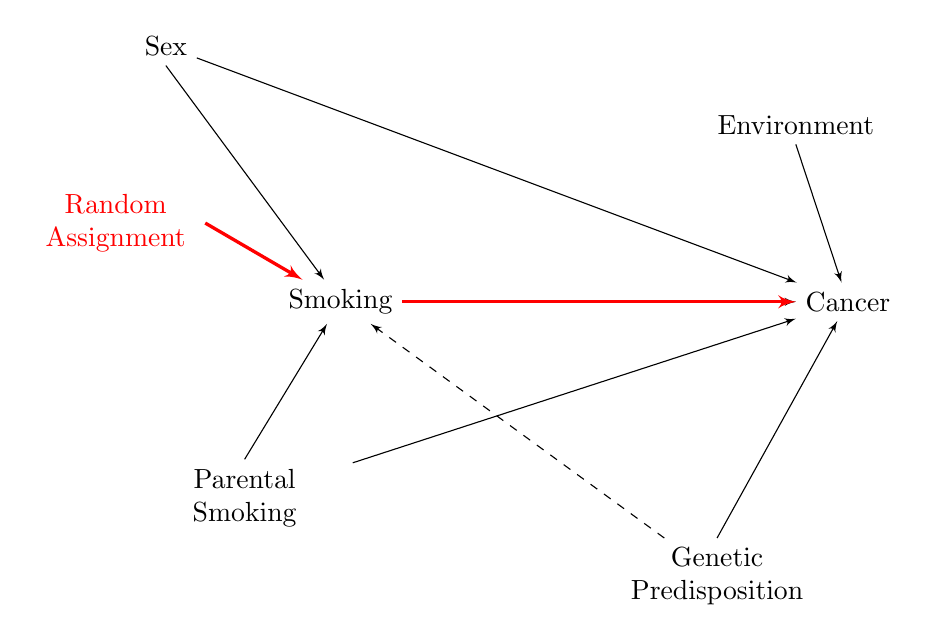
\begin{tikzpicture}[>=latex',circ/.style={draw, shape=circle, node distance=5cm, line width=1.5pt}]
    \draw[->] (0,0) node[left] (X) {Smoking} -- (5,0) node[right] (Y) {Cancer};
    \draw[->] (-3,3) node[above] (Z) {Sex} -- (X);
    \draw[->] (Z) -- (Y);
    \draw[->] (5,2) node[above] (A) {Environment} -- (Y);
    \draw[->] (4,-3) node[below, text width=3cm, align=center] (E) {Genetic\\Predisposition} -- (Y);
    \draw[->] (-2, -2) node[below, text width=2.5cm, align=center] (W) {Parental\\Smoking} -- (X);
    \draw[->] (W) -- (Y);
    \draw[->, dashed] (E) -- (X);
    
    \draw<2->[->, very thick, color=red] (-2.5,1) node[left, color=red, text width=2cm, align=center] (Tr) {Random\\Assignment} -- (X);
    \draw<2->[->, very thick, color=red] (X) -- (Y);
\end{tikzpicture}
\end{center}
\end{frame}

\questions



\frame{

\large
\centering
Does randomization \textit{guarantee balance}? Does it work every time?

\vspace{1em}

\only<2->{What happens if there is imbalance? How would we know?}
}


\frame{

\frametitle{Balance Testing I}

\begin{itemize}\itemsep0.5em
\item Analysis of experiments assumes that randomization produces covariate balance
\item<2-> But this is only true \textit{in expectation}
\item<3-> If we find covariate imbalance, we can:
	\begin{itemize}
	\item Ignore it
	\item Condition on imbalanced covariates
	\end{itemize}
\end{itemize}

}

\frame{

\frametitle{Balance Testing II}

There are three basic ways to detect covariate imbalance:

\begin{enumerate}\itemsep1em
\item Regressing treatment assignment on covariates
\item Conducting t-tests for each covariate across experimental groups
\item Examining covariate means visually
\end{enumerate}

}



\frame{
\frametitle{Experimental Analysis}
\small
\begin{itemize}
\item The statistic of interest in an experiment is the \textit{sample average treatment effect} (SATE)
\item If our sample is \textit{representative}, then this provides an estimate of the population average treatment (PATE)
\item This boils down to being a mean-difference between two groups:
	\begin{equation}
	SATE = \frac{1}{n_1}\sum Y_{1i} - \frac{1}{n_0}\sum Y_{0i}
	\end{equation}
\item<2->The Neyman--Rubin logic only works for \textit{means}\footnote{But not medians, etc.}
\end{itemize}
}



\frame{

\frametitle{Computation of Effects}

\begin{itemize}\itemsep0.5em
\item In practice we often estimate SATE using t-tests, ANOVA, or OLS regression
\item These are all basically equivalent
\item<2-> Reasons to choose one procedure over another:
	\begin{itemize}
	\item<2-> Disciplinary norms
	\item<3-> Ease of interpretation
	\item<4-> Flexibility for >2 treatment conditions
	\end{itemize}
\end{itemize}



}

\frame[label=tidy]{

\frametitle{Experimental Data Tidying}

An experimental data structure looks like:

\small

\begin{center}
\begin{tabular}{ccc}
\texttt{unit} & \texttt{treatment} & \texttt{outcome} \\ \hline 
1 & 0 & 13 \\
2 & 0 & 6 \\
3 & 0 & 4 \\
4 & 0 & 5 \\
5 & 1 & 3 \\
6 & 1 & 1 \\
7 & 1 & 10 \\
8 & 1 & 9 \\ \hline
\end{tabular}
\end{center}

}

\frame{

\frametitle{Experimental Data Tidying}

Sometimes it looks like this instead, which is bad:

\small

\begin{center}
\begin{tabular}{cccc}
\texttt{unit} & \texttt{treatment} & \texttt{outcome0}  & \texttt{outcome1} \\ \hline 
1 & 0 & 13 & . \\
2 & 0 & 6 & . \\
3 & 0 & 4 & . \\
4 & 0 & 5 & . \\
5 & 1 & . & 3 \\
6 & 1 & . & 1 \\
7 & 1 & . & 10 \\
8 & 1 & . & 9 \\ \hline
\end{tabular}
\end{center}

}

\againframe{tidy}


\frame{

\frametitle{Experimental Data Tidying}

Sometimes it looks like this instead, which is even worse:

\small

\begin{center}
\begin{tabular}{cccc}
\texttt{unit} & \texttt{treatment} & \texttt{outcome0}  & \texttt{outcome1} \\ \hline 
1 & . & 13 & . \\
2 & . & 6 & . \\
3 & . & 4 & . \\
4 & . & 5 & . \\
5 & . & . & 3 \\
6 & . & . & 1 \\
7 & . & . & 10 \\
8 & . & . & 9 \\ \hline
\end{tabular}
\end{center}

}

\againframe{tidy}

\frame{

\frametitle{Experimental Data Tidying}

Sometimes it looks like this instead, which is even more worse:

\small

\begin{center}
\begin{tabular}{ccccc}
\texttt{unit} & \texttt{treatment} & \texttt{outcome0}  & \texttt{outcome1} & \texttt{order} \\ \hline 
1 & . & 13 & 6 & 0,1\\
2 & . & 6 & 8 & 0,1\\
3 & . & 4 & 2 & 0,1\\
4 & . & 5 & 1 & 0,1\\
5 & . & 9 & 3 & 1,0\\
6 & . & 4 & 1 & 1,0\\
7 & . & 2 & 10 & 1,0\\
8 & . & 8 & 9 & 1,0\\ \hline
\end{tabular}
\end{center}

}

\againframe{tidy}






\begin{frame}[fragile]

\frametitle{Computation of Effects in Stata}

Stata:\small
\begin{verbatim}
ttest outcome, by(treatment)
reg outcome i.treatment
\end{verbatim}

R:\small
\begin{verbatim}
t.test(outcome ~ treatment, data = data)
lm(outcome ~ factor(treatment), data = data)
\end{verbatim}

\end{frame}


\questions




\frame{
\frametitle{SATE Variance Estimation}
	\small
\begin{itemize}\itemsep0.5em
\item We don't just care about the size of the SATE. We also want to know whether it is significantly different from zero (i.e., different from no effect/difference)
\item To know that, we need to estimate the \textit{variance} of the SATE
\item The variance is influenced by:
	\begin{itemize}
	\item Total sample size
	\item Variance of the outcome, $Y$
	\item Relative size of each treatment group
	\end{itemize}
\end{itemize}
}


\frame{
\frametitle{SATE Variance Estimation}
	\small
\begin{itemize}\itemsep0.5em
\item Formula for the variance of the SATE is:\\
$\widehat{Var}(SATE) = \dfrac{\widehat{Var}(Y_0)}{n_0} + \dfrac{\widehat{Var}(Y_1)}{n_1}$

	\begin{itemize}
	\item $\widehat{Var}(Y_0)$ is control group variance
	\item $\widehat{Var}(Y_1)$ is treatment group variance
	\end{itemize}

\item We often express this as the \textit{standard error} of the estimate:\\
$\widehat{SE}_{SATE} = \sqrt{\frac{\widehat{Var}(Y_0)}{n_0} + \frac{\widehat{Var}(Y_1)}{n_1}}$
\end{itemize}
}


\frame{

\frametitle{Intuition about Variance}

\begin{itemize}\itemsep0.5em
\item Bigger sample $\rightarrow$ smaller SEs
\item Smaller variance $\rightarrow$ smaller SEs
\item Efficient use of sample size:
	\begin{itemize}
	\item When treatment group variances equal, equal sample sizes are most efficient
	\item When variances differ, sample units are better allocated to the group with higher variance in \emph{Y}
	\end{itemize}
\end{itemize}

}


\frame{
	\frametitle{Important considerations}
	\begin{itemize}\itemsep0.5em
		\item Required sample size depends on $SATE$ and $Var(Y)$
		\item<2-> In large populations, population size is irrelevant
		\item<3-> In small populations, precision is influenced by the proportion of population sampled
		\item<4-> In anything other than an SRS, sample size calculation is more difficult
		\item<5-> Most research assumes SRS even though a more complex design is actually used
		\item<6-> Sample size needed to obtain a precise estimate of SATE is always going to be twice as large as needed to obtain an precise estimate of $\bar{Y}$
	\end{itemize}
}

\frame{
	\frametitle{Estimating sample size}
	What precision (margin of error) do we want?
	\begin{itemize}
		\item $p$ +/- 5 percentage points: $SE = 0.025$
			\begin{equation}
			n = \frac{0.25}{0.000625} = 400
			\end{equation}
		\item<2-> $p$ +/- 2 percentage points: $SE = 0.01$
			\begin{equation}
			n = \frac{0.25}{0.01^2} = \frac{0.25}{0.0001} = 2500
			\end{equation}
		\item<3-> $p$ +/- 0.5 percentage points: $SE = 0.0025$
			\begin{equation}
			n = \frac{0.25}{0.00000625} = 40,000
			\end{equation}
	\end{itemize}
}


\frame{

\frametitle{Statistical Power}

\begin{itemize}\itemsep0.5em
\item Power analysis is used to determine sample size before conducting an experiment

\item Type I and Type II Errors

\begin{center}
\begin{tabular}{lcc}
\toprule
& $H_0$ False & $H_0$ True \\ 
& ($|ATE| > 0$) & ($ATE = 0$) \\ \midrule
Reject $H_0$ & \textbf{True positive} & Type I Error \\
Accept $H_0$ & Type II Error & True zero \\ \bottomrule
\end{tabular}
\end{center}

	\begin{itemize}
	\item True positive rate ($1-\kappa$) is power
	\item False positive rate is the significance threshold ($\alpha$)
	\end{itemize}

\end{itemize}
}



\frame{

\frametitle{Doing a Power Analysis}

\begin{itemize}
\item $\mu$, Treatment group mean outcomes
\item $N$, Sample size
\item $\sigma$, Outcome variance
\item $\alpha$ Statistical significance threshold
\item $\phi$, a sampling distribution
\end{itemize}

$Power = \phi\left( \frac{|\mu_1 - \mu_0|\sqrt{N}}{2\sigma} - \phi^{-1}\left( 1 - \frac{\alpha}{2} \right) \right)$

}



\frame{
\frametitle{Intuition about Power}

Minimum detectable effect is the smallest effect we could detect given sample size, ``true'' ATE, variance of outcome measure, power ($1-\kappa$), and $\alpha$.\\

\vspace{1em}

\only<2->{In essence: some non-zero effect sizes are not detectable by a study of a given sample size.}

\vspace{1em}

\only<3->{In underpowered study, we will be unlikely to detect true small effects. And most effects are small! \footnote{Gelman, A. and Weakliem, D. 2009. ``Of Beauty, Sex and Power.'' \textit{American Scientist} 97(4): 310--16}}

}


\frame{

\frametitle{Intuition about Power}

\begin{itemize}\itemsep1em
\item It can help to think in terms of ``standardized effect sizes''
\item Intuition: How large is the effect in standard deviations of the outcome?
	\begin{itemize}
	\item Know if effects are large or small
	\item Compare effects across studies
	\end{itemize}
\item<2-> Cohen's $d$:\\ $d = \frac{\bar{x}_1 - \bar{x}_0}{s}$, where
$s = \sqrt{\frac{(n_1 - 1)s_1^2 + (n_0 - 1)s_0^2}{n_1 + n_0 - 2}}$
\item<3-> Small: 0.2; Medium: 0.5; Large: 0.8
\end{itemize}

}

\frame{
\frametitle{Intuition about Power}

\begin{center}
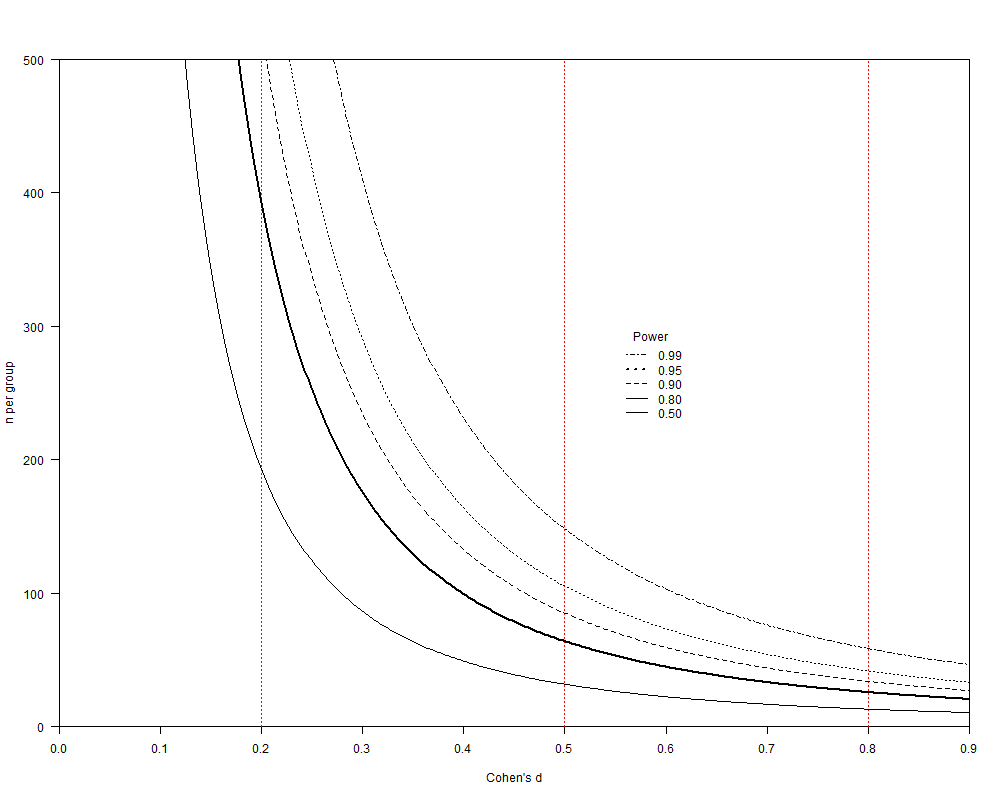
\includegraphics[height=0.8\textheight, trim = 0in 0in 0in 0.5in , clip]{images/power}
\end{center}

}


\begin{frame}[fragile]

\frametitle{Power analysis in R}
\small
\begin{verbatim}
power.t.test(
  # sample size (leave blank!)
  n = ,
  
  # minimum detectable effect size
  delta = 0.4, sd = 1,
  
  # alpha and power (1-kappa)
  sig.level = 0.05, power = 0.8,
  
  # two-tailed vs. one-tailed test
  alternative = "two.sided"
)
\end{verbatim}
\end{frame}


\begin{frame}[fragile]

\frametitle{Power analysis in Stata}
\small
\begin{verbatim}
power twomeans 0, diff(0.2)

// for multiple values of 
forvalues i = 0.1 (0.1) 1.0 {
    power twomeans 0, diff(`i')
}

// using raw effect sizes and standard deviations
power twomeans 0 0.5, sd1(.5) sd2(.7)

// adjusting alpha or power
power twomeans 0, diff(0.2) alpha(0.10) power(0.7)
\end{verbatim}
\end{frame}



\begin{frame}

\frametitle{Increasing/Decreasing Power}

\begin{columns}
\begin{column}{0.5\textwidth}
\begin{block}{Increases Power}
\begin{itemize}\itemsep1em
\item Bigger sample
\item Precise measures
\item Covariates?
\end{itemize}
\end{block}
\end{column}

\begin{column}{0.5\textwidth}
\begin{block}{Decreases Power}
\begin{itemize}\itemsep1em
\item Attrition
\item Noncompliance
\item Clustering
\end{itemize}
\end{block}
\end{column}
\end{columns}

\end{frame}


\frame{

\frametitle{Aside: Complex Designs}

\small

\begin{itemize}
\item An experiment can have any number of conditions
	\begin{itemize}\footnotesize
	\item Up to the limits of sample size
	\item More than 8--10 conditions is typically unwieldy
	\end{itemize}
\item Typically analyze complex designs using ANOVA or regression, but we are still ultimately interested in pairwise comparisons to estimates SATEs
	\begin{itemize}\footnotesize
	\item Treatment--treatment, or treatment-control
	\item Without control group, we don't know which treatment(s) affected the outcome
	\end{itemize}
\end{itemize}

}


\frame{}


\frame{
\frametitle{{\large \textit{Survey}-experiments, specifically}}

\small

\begin{itemize}
\item Everything so far applies to any kind of experiment
\item<2-> A survey experiment is just an experiment that occurs in a survey context
	\begin{itemize}
	\item As opposed to in the field or in a laboratory
	\end{itemize}
\item<3-> Sometimes a distinction is made between survey and online experiments
\item<4-> Lots of common paradigms for survey experiments (later)
\end{itemize}
}

\questions

\frame{

\frametitle{Factorial Designs}

\begin{itemize}\itemsep1em
\item The two-condition experiment is a stylized ideal

\item An experiment can have any number of conditions
	\begin{itemize}\footnotesize
	\item Up to the limits of sample size
	\item More than 8--10 conditions is typically unwieldy
	\end{itemize}

\item Three ``flavors'':
	\begin{itemize}
	\item Multiple conditions in a single factor
	\item Multiple fully \textit{crossed} factors
	\item Partially crossed (``fractional factorial'') designs
	\end{itemize}

\item Regression methods provide a generalizable tool for causal inference in such designs
\end{itemize}
}

\begin{frame}
\begin{center}
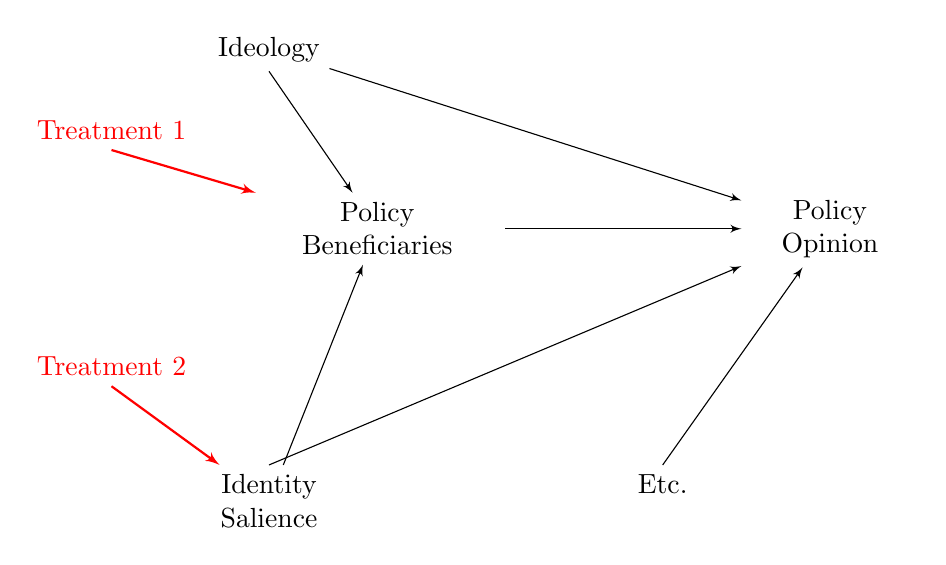
\begin{tikzpicture}[>=latex',circ/.style={draw, shape=circle, node distance=5cm, line width=1.5pt}]
    \draw (0,0) node[left, text width=3cm, align=center] (X) {Policy\\Beneficiaries};
    \draw[->] (X) -- (3,0) node[right, text width=2cm, align=center] (Y) {Policy\\Opinion};
    \draw[->] (-3,2) node[above] (Z) {Ideology} -- (X);
    \draw[->] (Z) -- (Y);
    \draw[->] (2,-3) node[below, text width=3cm, align=center] (E) {Etc.} -- (Y);
    \draw[->] (-3, -3) node[below, text width=2.5cm, align=center] (W) {Identity Salience} -- (Y);
    \draw[->] (W) -- (X);
    \draw<2->[->,thick,red] (-5,1) node[above] (T1) {Treatment 1} -- (X);
    \draw<2->[->,thick,red] (-5,-2) node[above] (T1) {Treatment 2} -- (W);
\end{tikzpicture}
\end{center}
\end{frame}


\frame{
	\frametitle{{\normalsize Example\footnote{Transue. 2007. ``Identity Salience, Identity Acceptance, and Racial Policy Attitudes: {American} National Identity as a Uniting Force.'' \textit{American Journal of Political Science} 51(1): 78--91.}}}
	

\begin{itemize}\itemsep1em
\item \only<1,3>{How close do you feel to your ethnic or racial group?}\only<2,4>{How close do you feel to other Americans?}
\item \only<1-2>{Some people have said that taxes need to be raised to take care of pressing national needs. How willing would you be to have your taxes raised to improve education in public schools?}\only<3-4>{Some people have said that taxes need to be raised to take care of pressing national needs. How willing would you be to have your taxes raised to improve educational opportunities for minorities?}
\end{itemize}
	
}


\frame{

\frametitle{2x2 Factorial Design}

\only<1>{
\begin{center}
\begin{tabular}{lr}
Condition &  \\ \midrule
Educ. for Minorities & $Y_1$ \\
Schools & $Y_0$ \\ \bottomrule
\end{tabular}
\end{center}
}

\only<2>{
\begin{center}
\begin{tabular}{lrr}
Condition & Americans & Own Race \\ \midrule
Educ. for Minorities & $Y_{1,0}$ & $Y_{1,1}$ \\
Schools & $Y_{0,0}$ & $Y_{0,1}$ \\ \bottomrule
\end{tabular}
\end{center}
}

}


\frame{

\frametitle{Two ways to \textit{parameterize} this}

Dummy variable regression (i.e., treatment--control CATEs):

$Y = \beta_0 + \beta_1 X_{0,1} + \beta_2 X_{1,0} + \beta_3 X_{1,1} + \epsilon$

\vspace{1em}

Interaction effects (i.e., treatment--treatment CATEs):

$Y = \beta_0 + \beta_1 X1_{1} + \beta_2 X2_{1} + \beta_3 X1_1 * X2_1 + \epsilon$

\vspace{1em}

Use \texttt{margins} to extract marginal effects

}


\frame<1>[label=factorialconsiderations]{

\frametitle{Considerations}

\begin{itemize}\itemsep0.5em
\item Factorial designs can quickly become unwieldy and expensive
\item<2-> Need to consider what CATEs are of theoretical interest
	\begin{itemize}
	\item Treatment--control, pairwise
	\item Treatment--treatment, pairwise
	\item Marginal effects, averaging across other factors
	\item Comparison of merged conditions
	\end{itemize}
\end{itemize}

}

\frame{

\frametitle{Probably obvious, but\dots}

\footnotesize

\begin{center}
\begin{tabular}{cccc}
Factors & Conditions per factor & Total Conditions & $n$ \\ \midrule
1 & 2 & 2 & 400 \\ 
1 & 3 & 3 & 600 \\
1 & 4 & 4 & 800 \\
2 & 2 & 4 & 800 \\
2 & 3 & 6 & 1200 \\
2 & 4 & 8 & 1600 \\
3 & 3 & 9 & 1800 \\
3 & 4 & 12 & 2400 \\
4 & 4 & 16 & 3200 \\ \bottomrule
\end{tabular}
\end{center}

{\footnotesize Assumes power to detect a relatively small effect, but no consideration of multiple comparisons.}

}

\againframe{factorialconsiderations}

% marginal effects of factors are marginal across the set of levels of the other factors; if those factors aren't complete, then external validity problem


\questions


\appendix
\frame{}

\begin{frame}[fragile]

\frametitle{{\large Randomization Distribution}}

\tiny

\begin{verbatim}
# theoretical randomizations
onedraw <- function(eff=FALSE, dat = d) {
  r <- replicate(nrow(dat), sample(1:2,1))
  dat[cbind(1:nrow(dat),r)] <- NA
  if (eff) {
    return(mean(dat[,'y1'], na.rm=TRUE) -
           mean(dat[,'y0'], na.rm=TRUE) )
  } else {
    return(dat)
  }
}

onedraw() # one randomization
onedraw(TRUE) # one effect estimate

# simulate 2000 experiments from these data
x1 <- replicate(2000, onedraw(TRUE))
hist(x1, col=rgb(1,0,0,.5), border='white')
abline(v=-2, lwd=3, col='red') # true effect
\end{verbatim}

\end{frame}


\frame{}


\frame{

\large\centering
One way to avoid covariate imbalance and improve statistical power is \textbf{block randomization}.

}

\frame{

\frametitle{Block Randomization I}

{\small \textbf{Stratification:Sampling::Blocking:Experiments}}

\small

\begin{itemize}\itemsep0.5em
\item<2-> Basic idea: randomization occurs within strata defined before treatment assignment
\item<3-> CATE is estimate for each stratum; aggregated to SATE
\item<4-> Why?
	\begin{itemize}
	\item Eliminate chance imbalances
	\item Optimized for estimating CATEs
	\item More precise SATE estimate
	\end{itemize}
\end{itemize}

}

\begin{frame}[fragile]

\begin{center}
\begin{tabular}{lcccccccc}
Exp. & \multicolumn{4}{c}{Control} & \multicolumn{4}{c}{Treatment} \\ \midrule
1 & M & M & M & M & F & F & F & F \\
2 & M & M & M & F & M & F & F & F \\
3 & M & M & F & F & M & M & F & F \\
4 & M & F & F & F & M & M & M & F \\
5 & F & F & F & F & M & M & M & M \\ \bottomrule
\end{tabular}
\end{center}

\end{frame}

\frame{

\begin{center}

\begin{tabular}{rrrr}
Obs. & $X_{1i}$ & $X_{2i}$ & $D_i$ \\ \midrule
1 & Male & Old & 0 \\
2 & Male & Old & 1 \\  \midrule
3 & Male & Young & 1 \\
4 & Male & Young & 0 \\ \midrule
5 & Female & Old & 1 \\
6 & Female & Old & 0 \\ \midrule
7 & Female & Young & 0 \\
8 & Female & Young & 1 \\ \bottomrule
\end{tabular}
\end{center}

}

\frame[label=blocking2]{

\frametitle{Block Randomization II}

\begin{itemize}
\item Blocking ensures ignorability of all covariates used to construct the blocks
\item Incorporates covariates explicitly into the \textit{design}
\item<2-> When is blocking \textit{statistically} useful?
	\begin{itemize}
	\item<3-> If those covariates affect values of potential outcomes, blocking reduces the variance of the SATE
	\item<4-> Most valuable in small samples
	\item<5-> Not valuable if all blocks have similar potential outcomes
	\end{itemize}
\end{itemize}

}



\frame{

\frametitle{Statistical Properties I}

\small

Complete randomization:\\
$$SATE = \frac{1}{n_1}\sum Y_{1i} - \frac{1}{n_0}\sum Y_{0i}$$

\vspace{2em}

Block randomization:\\
$$SATE_{blocked} = \sum_{1}^{J} \left( \dfrac{n_j}{n} \right)  (\widehat{CATE}_j)$$

}


\frame{

\begin{center}

\begin{tabular}{rrrrrr}
Obs. & $X_{1i}$ & $X_{2i}$ & $D_i$ & $Y_i$ & CATE \\ \midrule
1 & Male & Old & 0 & 5 & \multirow{2}{*}{\onslide<2->{5}} \\
2 & Male & Old & 1 & 10 \\  \midrule
3 & Male & Young & 1 & 4 & \multirow{2}{*}{\onslide<3->{3}} \\
4 & Male & Young & 0 & 1 \\ \midrule
5 & Female & Old & 1 & 6 & \multirow{2}{*}{\onslide<4->{4}} \\
6 & Female & Old & 0 & 2 \\ \midrule
7 & Female & Young & 0 & 6 & \multirow{2}{*}{\onslide<5->{3}} \\
8 & Female & Young & 1 & 9 \\ \bottomrule
\end{tabular}
\end{center}

}

\frame{

\frametitle{SATE Estimation}

\begin{align*}
SATE &= \left(\dfrac{2}{8}*5\right) + \left(\dfrac{2}{8}*3\right) + \left(\dfrac{2}{8}*4\right) + \left(\dfrac{2}{8}*3\right) \\ \vspace{1em}
&= 3.75
\end{align*}

\onslide<2->{The blocked and unblocked estimates are the same here because $Pr(Treatment)$ is constant across blocks and blocks are all the same size.}

}

\frame{

\frametitle{SATE Estimation}

\small

\begin{itemize}
\item We can use weighted regression to estimate this in an OLS framework
\item Weights are the inverse prob. of being treated w/in block
\begin{itemize}
\item Pr(Treated) by block: $p_{ij} = Pr(D_i = 1 | J=j) $
\item Weight (Treated): $ w_{ij} = \dfrac{1}{p_{ij}} $
\item Weight (Control): $ w_{ij} = \dfrac{1}{1-p_{ij}} $
\end{itemize}
\end{itemize}

}


\frame{

\frametitle{Statistical Properties II}

\small

Complete randomization:\\
$$\widehat{SE}_{SATE} = \sqrt{\dfrac{\widehat{Var}(Y_0)}{n_0} + \dfrac{\widehat{Var}(Y_1)}{n_1}}$$

\vspace{1em}

Block randomization:\\
$$\widehat{SE}_{SATE_{blocked}} = \sqrt{\sum_{1}^{J} \left( \dfrac{n_j}{n} \right)^2  \widehat{Var}{(SATE_j)}}$$

\only<2->{When is the blocked design more efficient?}

}


\frame{

\frametitle{Practicalities}

\begin{itemize}\itemsep0.5em
\item Blocked randomization only works in exactly the same situations where stratified sampling works
	\begin{itemize}
	\item Need to observe covariates pre-treatment in order to block on them
	\item Work best in a panel context
	\end{itemize}
\item In a single cross-sectional design that might be challenging
	\begin{itemize}
	\item Some software can block ``on the fly''
	\end{itemize}
\end{itemize}


}


\end{document}
